% Options for packages loaded elsewhere
\PassOptionsToPackage{unicode}{hyperref}
\PassOptionsToPackage{hyphens}{url}
\documentclass[
]{article}
\usepackage{xcolor}
\usepackage[margin=1in]{geometry}
\usepackage{amsmath,amssymb}
\setcounter{secnumdepth}{-\maxdimen} % remove section numbering
\usepackage{iftex}
\ifPDFTeX
  \usepackage[T1]{fontenc}
  \usepackage[utf8]{inputenc}
  \usepackage{textcomp} % provide euro and other symbols
\else % if luatex or xetex
  \usepackage{unicode-math} % this also loads fontspec
  \defaultfontfeatures{Scale=MatchLowercase}
  \defaultfontfeatures[\rmfamily]{Ligatures=TeX,Scale=1}
\fi
\usepackage{lmodern}
\ifPDFTeX\else
  % xetex/luatex font selection
\fi
% Use upquote if available, for straight quotes in verbatim environments
\IfFileExists{upquote.sty}{\usepackage{upquote}}{}
\IfFileExists{microtype.sty}{% use microtype if available
  \usepackage[]{microtype}
  \UseMicrotypeSet[protrusion]{basicmath} % disable protrusion for tt fonts
}{}
\makeatletter
\@ifundefined{KOMAClassName}{% if non-KOMA class
  \IfFileExists{parskip.sty}{%
    \usepackage{parskip}
  }{% else
    \setlength{\parindent}{0pt}
    \setlength{\parskip}{6pt plus 2pt minus 1pt}}
}{% if KOMA class
  \KOMAoptions{parskip=half}}
\makeatother
\usepackage{color}
\usepackage{fancyvrb}
\newcommand{\VerbBar}{|}
\newcommand{\VERB}{\Verb[commandchars=\\\{\}]}
\DefineVerbatimEnvironment{Highlighting}{Verbatim}{commandchars=\\\{\}}
% Add ',fontsize=\small' for more characters per line
\usepackage{framed}
\definecolor{shadecolor}{RGB}{248,248,248}
\newenvironment{Shaded}{\begin{snugshade}}{\end{snugshade}}
\newcommand{\AlertTok}[1]{\textcolor[rgb]{0.94,0.16,0.16}{#1}}
\newcommand{\AnnotationTok}[1]{\textcolor[rgb]{0.56,0.35,0.01}{\textbf{\textit{#1}}}}
\newcommand{\AttributeTok}[1]{\textcolor[rgb]{0.13,0.29,0.53}{#1}}
\newcommand{\BaseNTok}[1]{\textcolor[rgb]{0.00,0.00,0.81}{#1}}
\newcommand{\BuiltInTok}[1]{#1}
\newcommand{\CharTok}[1]{\textcolor[rgb]{0.31,0.60,0.02}{#1}}
\newcommand{\CommentTok}[1]{\textcolor[rgb]{0.56,0.35,0.01}{\textit{#1}}}
\newcommand{\CommentVarTok}[1]{\textcolor[rgb]{0.56,0.35,0.01}{\textbf{\textit{#1}}}}
\newcommand{\ConstantTok}[1]{\textcolor[rgb]{0.56,0.35,0.01}{#1}}
\newcommand{\ControlFlowTok}[1]{\textcolor[rgb]{0.13,0.29,0.53}{\textbf{#1}}}
\newcommand{\DataTypeTok}[1]{\textcolor[rgb]{0.13,0.29,0.53}{#1}}
\newcommand{\DecValTok}[1]{\textcolor[rgb]{0.00,0.00,0.81}{#1}}
\newcommand{\DocumentationTok}[1]{\textcolor[rgb]{0.56,0.35,0.01}{\textbf{\textit{#1}}}}
\newcommand{\ErrorTok}[1]{\textcolor[rgb]{0.64,0.00,0.00}{\textbf{#1}}}
\newcommand{\ExtensionTok}[1]{#1}
\newcommand{\FloatTok}[1]{\textcolor[rgb]{0.00,0.00,0.81}{#1}}
\newcommand{\FunctionTok}[1]{\textcolor[rgb]{0.13,0.29,0.53}{\textbf{#1}}}
\newcommand{\ImportTok}[1]{#1}
\newcommand{\InformationTok}[1]{\textcolor[rgb]{0.56,0.35,0.01}{\textbf{\textit{#1}}}}
\newcommand{\KeywordTok}[1]{\textcolor[rgb]{0.13,0.29,0.53}{\textbf{#1}}}
\newcommand{\NormalTok}[1]{#1}
\newcommand{\OperatorTok}[1]{\textcolor[rgb]{0.81,0.36,0.00}{\textbf{#1}}}
\newcommand{\OtherTok}[1]{\textcolor[rgb]{0.56,0.35,0.01}{#1}}
\newcommand{\PreprocessorTok}[1]{\textcolor[rgb]{0.56,0.35,0.01}{\textit{#1}}}
\newcommand{\RegionMarkerTok}[1]{#1}
\newcommand{\SpecialCharTok}[1]{\textcolor[rgb]{0.81,0.36,0.00}{\textbf{#1}}}
\newcommand{\SpecialStringTok}[1]{\textcolor[rgb]{0.31,0.60,0.02}{#1}}
\newcommand{\StringTok}[1]{\textcolor[rgb]{0.31,0.60,0.02}{#1}}
\newcommand{\VariableTok}[1]{\textcolor[rgb]{0.00,0.00,0.00}{#1}}
\newcommand{\VerbatimStringTok}[1]{\textcolor[rgb]{0.31,0.60,0.02}{#1}}
\newcommand{\WarningTok}[1]{\textcolor[rgb]{0.56,0.35,0.01}{\textbf{\textit{#1}}}}
\usepackage{graphicx}
\makeatletter
\newsavebox\pandoc@box
\newcommand*\pandocbounded[1]{% scales image to fit in text height/width
  \sbox\pandoc@box{#1}%
  \Gscale@div\@tempa{\textheight}{\dimexpr\ht\pandoc@box+\dp\pandoc@box\relax}%
  \Gscale@div\@tempb{\linewidth}{\wd\pandoc@box}%
  \ifdim\@tempb\p@<\@tempa\p@\let\@tempa\@tempb\fi% select the smaller of both
  \ifdim\@tempa\p@<\p@\scalebox{\@tempa}{\usebox\pandoc@box}%
  \else\usebox{\pandoc@box}%
  \fi%
}
% Set default figure placement to htbp
\def\fps@figure{htbp}
\makeatother
\setlength{\emergencystretch}{3em} % prevent overfull lines
\providecommand{\tightlist}{%
  \setlength{\itemsep}{0pt}\setlength{\parskip}{0pt}}
\usepackage{bookmark}
\IfFileExists{xurl.sty}{\usepackage{xurl}}{} % add URL line breaks if available
\urlstyle{same}
\hypersetup{
  pdftitle={Lab 2 - Aprendizaje No Supervisado},
  pdfauthor={Grupo 9},
  hidelinks,
  pdfcreator={LaTeX via pandoc}}

\title{Lab 2 - Aprendizaje No Supervisado}
\author{Grupo 9}
\date{February 23, 2026}

\begin{document}
\maketitle

\section{1. Clustering}\label{clustering}

\subsection{1.1 Carga y exploración inicial del
dataset}\label{carga-y-exploraciuxf3n-inicial-del-dataset}

\begin{Shaded}
\begin{Highlighting}[]
\NormalTok{movies }\OtherTok{\textless{}{-}} \FunctionTok{read.csv}\NormalTok{(}\StringTok{"data/movies\_2026.csv"}\NormalTok{)}
\FunctionTok{summary}\NormalTok{(movies)}
\end{Highlighting}
\end{Shaded}

\begin{verbatim}
##        id              budget             genres            homePage        
##  Min.   :      5   Min.   :        0   Length:19883       Length:19883      
##  1st Qu.: 146220   1st Qu.:        0   Class :character   Class :character  
##  Median : 869623   Median :        0   Mode  :character   Mode  :character  
##  Mean   : 902240   Mean   :  9413280                                        
##  3rd Qu.:1589603   3rd Qu.:  1000000                                        
##  Max.   :1627166   Max.   :380000000                                        
##                                                                             
##  productionCompany  productionCompanyCountry productionCountry 
##  Length:19883       Length:19883             Length:19883      
##  Class :character   Class :character         Class :character  
##  Mode  :character   Mode  :character         Mode  :character  
##                                                                
##                                                                
##                                                                
##                                                                
##     revenue             runtime         video           director        
##  Min.   :0.000e+00   Min.   :  0.00   Mode :logical   Length:19883      
##  1st Qu.:0.000e+00   1st Qu.: 10.00   FALSE:19313     Class :character  
##  Median :0.000e+00   Median : 86.00   TRUE :84        Mode  :character  
##  Mean   :2.879e+07   Mean   : 66.09   NA's :486                         
##  3rd Qu.:3.306e+05   3rd Qu.:103.00                                     
##  Max.   :2.847e+09   Max.   :750.00                                     
##                                                                         
##     actors          actorsPopularity   actorsCharacter    originalTitle     
##  Length:19883       Length:19883       Length:19883       Length:19883      
##  Class :character   Class :character   Class :character   Class :character  
##  Mode  :character   Mode  :character   Mode  :character   Mode  :character  
##                                                                             
##                                                                             
##                                                                             
##                                                                             
##     title           originalLanguage     popularity        releaseDate       
##  Length:19883       Length:19883       Min.   :0.000e+00   Length:19883      
##  Class :character   Class :character   1st Qu.:5.460e-02   Class :character  
##  Mode  :character   Mode  :character   Median :8.502e+00   Mode  :character  
##                                        Mean   :2.625e+01                     
##                                        3rd Qu.:2.224e+01                     
##                                        Max.   :1.147e+04                     
##                                                                              
##     voteAvg         voteCount        genresAmount    productionCoAmount
##  Min.   : 0.000   Min.   :    0.0   Min.   : 0.000   Min.   : 0.000    
##  1st Qu.: 0.000   1st Qu.:    0.0   1st Qu.: 1.000   1st Qu.: 0.000    
##  Median : 5.400   Median :    6.0   Median : 2.000   Median : 1.000    
##  Mean   : 3.837   Mean   :  675.9   Mean   : 1.949   Mean   : 1.973    
##  3rd Qu.: 6.800   3rd Qu.:  423.0   3rd Qu.: 3.000   3rd Qu.: 3.000    
##  Max.   :10.000   Max.   :30788.0   Max.   :16.000   Max.   :89.000    
##                                                                        
##  productionCountriesAmount  actorsAmount    castWomenAmount  castMenAmount   
##  Min.   :  0.00            Min.   :     0   Min.   :     0   Min.   :     0  
##  1st Qu.:  1.00            1st Qu.:     3   1st Qu.:     0   1st Qu.:     0  
##  Median :  1.00            Median :     9   Median :     2   Median :     3  
##  Mean   :  1.23            Mean   :  1082   Mean   :  3517   Mean   :  8224  
##  3rd Qu.:  1.00            3rd Qu.:    21   3rd Qu.:     6   3rd Qu.:    12  
##  Max.   :155.00            Max.   :919590   Max.   :922162   Max.   :922017  
##                                             NA's   :37       NA's   :162     
##   releaseYear  
##  Min.   :1902  
##  1st Qu.:2013  
##  Median :2021  
##  Mean   :2017  
##  3rd Qu.:2025  
##  Max.   :2026  
##  NA's   :2
\end{verbatim}

El dataset contiene 19,883 películas con variables relacionadas a
presupuesto, ingresos, popularidad, votos, producción y elenco.\\
Se observan valores extremos en variables como \texttt{budget},
\texttt{revenue} y \texttt{actorsAmount}, lo que hace necesario
estandarizar antes de aplicar clustering.

\begin{center}\rule{0.5\linewidth}{0.5pt}\end{center}

\subsection{\texorpdfstring{1.2 Preprocesamiento de la variable
\texttt{genres}}{1.2 Preprocesamiento de la variable genres}}\label{preprocesamiento-de-la-variable-genres}

Se limpian los espacios y se separan los géneros múltiples.

\begin{Shaded}
\begin{Highlighting}[]
\NormalTok{movies }\OtherTok{\textless{}{-}}\NormalTok{ movies }\SpecialCharTok{\%\textgreater{}\%}
  \FunctionTok{mutate}\NormalTok{(}\AttributeTok{genres =} \FunctionTok{gsub}\NormalTok{(}\StringTok{" }\SpecialCharTok{\textbackslash{}\textbackslash{}}\StringTok{| "}\NormalTok{, }\StringTok{"|"}\NormalTok{, genres))}

\NormalTok{movies\_long }\OtherTok{\textless{}{-}}\NormalTok{ movies }\SpecialCharTok{\%\textgreater{}\%}
  \FunctionTok{separate\_rows}\NormalTok{(genres, }\AttributeTok{sep =} \StringTok{"}\SpecialCharTok{\textbackslash{}\textbackslash{}}\StringTok{|"}\NormalTok{)}

\NormalTok{movies\_longs }\OtherTok{\textless{}{-}}\NormalTok{ movies\_long }\SpecialCharTok{\%\textgreater{}\%}
  \FunctionTok{separate\_rows}\NormalTok{(genres, }\AttributeTok{sep =} \StringTok{"}\SpecialCharTok{\textbackslash{}\textbackslash{}}\StringTok{s*}\SpecialCharTok{\textbackslash{}\textbackslash{}}\StringTok{|}\SpecialCharTok{\textbackslash{}\textbackslash{}}\StringTok{s*"}\NormalTok{)}
\end{Highlighting}
\end{Shaded}

Este paso permite tratar correctamente los múltiples géneros asociados a
cada película.

\begin{center}\rule{0.5\linewidth}{0.5pt}\end{center}

\subsection{1.3 Muestra para análisis}\label{muestra-para-anuxe1lisis}

Debido al tamaño del dataset, se toma una muestra de 5000 registros.

\begin{Shaded}
\begin{Highlighting}[]
\FunctionTok{set.seed}\NormalTok{(}\DecValTok{123}\NormalTok{)}
\NormalTok{sample\_movies }\OtherTok{\textless{}{-}}\NormalTok{ movies\_longs[}\FunctionTok{sample}\NormalTok{(}\FunctionTok{nrow}\NormalTok{(movies\_longs), }\DecValTok{5000}\NormalTok{), ]}
\end{Highlighting}
\end{Shaded}

Esto reduce el costo computacional sin afectar significativamente la
representatividad del análisis.

\begin{center}\rule{0.5\linewidth}{0.5pt}\end{center}

\subsection{1.4 Método del codo}\label{muxe9todo-del-codo}

Se seleccionan variables numéricas y se estandarizan.

\begin{Shaded}
\begin{Highlighting}[]
\NormalTok{numeric\_sample }\OtherTok{\textless{}{-}}\NormalTok{ sample\_movies[, }\FunctionTok{sapply}\NormalTok{(sample\_movies, is.numeric)]}
\NormalTok{numeric\_sample }\OtherTok{\textless{}{-}} \FunctionTok{na.omit}\NormalTok{(numeric\_sample)}

\FunctionTok{fviz\_nbclust}\NormalTok{(}
  \FunctionTok{scale}\NormalTok{(numeric\_sample),}
\NormalTok{  kmeans,}
  \AttributeTok{method =} \StringTok{"wss"}
\NormalTok{)}
\end{Highlighting}
\end{Shaded}

\pandocbounded{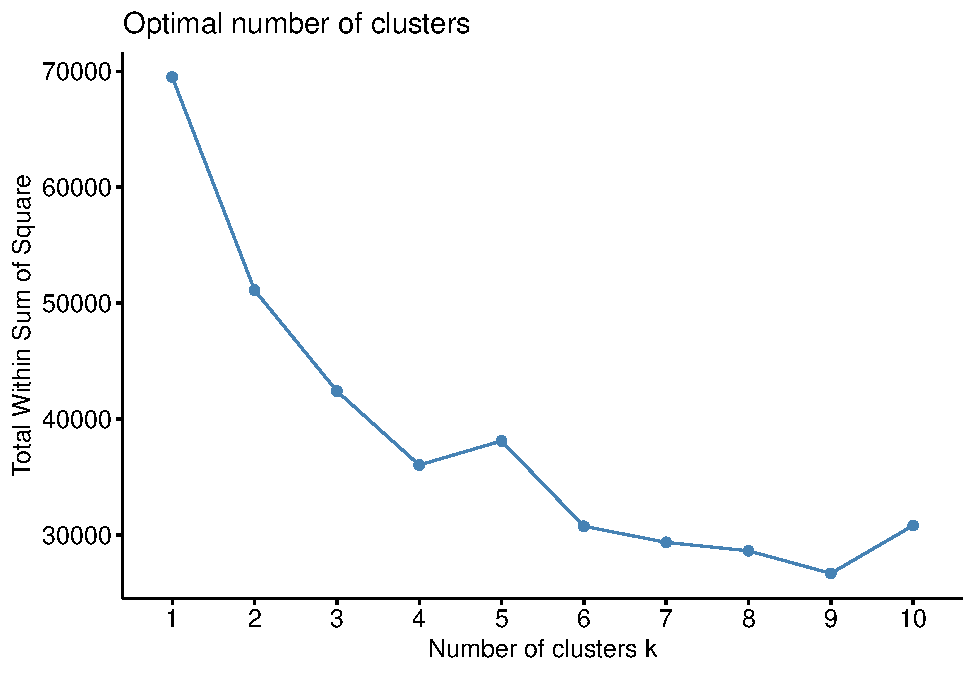
\includegraphics[keepaspectratio]{Lab2_files/figure-latex/metodo_codo-1.pdf}}

A partir de la gráfica del método del codo se observa un punto de
inflexión en \textbf{k = 4}, por lo que se determina trabajar con cuatro
clusters.

\begin{center}\rule{0.5\linewidth}{0.5pt}\end{center}

\subsection{1.5 Aplicación de algoritmos de
agrupamiento}\label{aplicaciuxf3n-de-algoritmos-de-agrupamiento}

Se utilizan K-means y Clustering Jerárquico con k = 4.

\begin{Shaded}
\begin{Highlighting}[]
\NormalTok{numeric\_vars }\OtherTok{\textless{}{-}}\NormalTok{ movies }\SpecialCharTok{\%\textgreater{}\%}
  \FunctionTok{select}\NormalTok{(popularity, budget, revenue, runtime, voteAvg,}
\NormalTok{         voteCount, genresAmount, productionCoAmount,}
\NormalTok{         productionCountriesAmount, actorsAmount,}
\NormalTok{         castWomenAmount, castMenAmount)}

\NormalTok{numeric\_vars }\OtherTok{\textless{}{-}} \FunctionTok{na.omit}\NormalTok{(numeric\_vars)}

\NormalTok{scaled\_data }\OtherTok{\textless{}{-}} \FunctionTok{scale}\NormalTok{(numeric\_vars)}

\CommentTok{\# K{-}means}
\FunctionTok{set.seed}\NormalTok{(}\DecValTok{123}\NormalTok{)}
\NormalTok{kmeans\_result }\OtherTok{\textless{}{-}} \FunctionTok{kmeans}\NormalTok{(scaled\_data, }\AttributeTok{centers =} \DecValTok{4}\NormalTok{, }\AttributeTok{nstart =} \DecValTok{25}\NormalTok{)}

\CommentTok{\# Jerárquico}
\NormalTok{dist\_matrix }\OtherTok{\textless{}{-}} \FunctionTok{dist}\NormalTok{(scaled\_data)}
\NormalTok{hc\_complete }\OtherTok{\textless{}{-}} \FunctionTok{hclust}\NormalTok{(dist\_matrix, }\AttributeTok{method =} \StringTok{"complete"}\NormalTok{)}
\NormalTok{hc\_clusters }\OtherTok{\textless{}{-}} \FunctionTok{cutree}\NormalTok{(hc\_complete, }\AttributeTok{k =} \DecValTok{4}\NormalTok{)}
\end{Highlighting}
\end{Shaded}

Se aplicaron ambos métodos para comparar calidad y distribución de
grupos.

\begin{center}\rule{0.5\linewidth}{0.5pt}\end{center}

\subsection{1.6 Evaluación con método de la
silueta}\label{evaluaciuxf3n-con-muxe9todo-de-la-silueta}

\begin{Shaded}
\begin{Highlighting}[]
\CommentTok{\# Silueta K{-}means}
\NormalTok{sil\_kmeans }\OtherTok{\textless{}{-}} \FunctionTok{silhouette}\NormalTok{(kmeans\_result}\SpecialCharTok{$}\NormalTok{cluster, }\FunctionTok{dist}\NormalTok{(scaled\_data))}
\FunctionTok{fviz\_silhouette}\NormalTok{(sil\_kmeans)}
\end{Highlighting}
\end{Shaded}

\begin{verbatim}
## Warning: `aes_string()` was deprecated in ggplot2 3.0.0.
## i Please use tidy evaluation idioms with `aes()`.
## i See also `vignette("ggplot2-in-packages")` for more information.
## i The deprecated feature was likely used in the factoextra package.
##   Please report the issue at <https://github.com/kassambara/factoextra/issues>.
## This warning is displayed once per session.
## Call `lifecycle::last_lifecycle_warnings()` to see where this warning was
## generated.
\end{verbatim}

\begin{verbatim}
##   cluster size ave.sil.width
## 1       1 9225          0.23
## 2       2  892          0.05
## 3       3  282          0.31
## 4       4 9322          0.55
\end{verbatim}

\pandocbounded{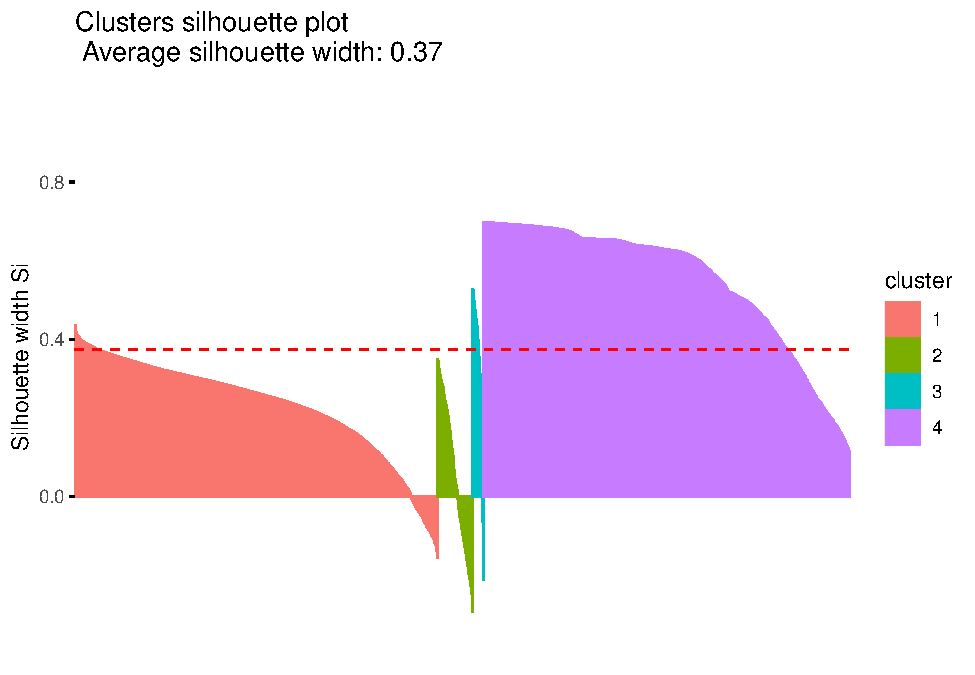
\includegraphics[keepaspectratio]{Lab2_files/figure-latex/silhouette-1.pdf}}

\begin{Shaded}
\begin{Highlighting}[]
\CommentTok{\# Silueta Jerárquico}
\NormalTok{sil\_hc }\OtherTok{\textless{}{-}} \FunctionTok{silhouette}\NormalTok{(hc\_clusters, }\FunctionTok{dist}\NormalTok{(scaled\_data))}
\FunctionTok{fviz\_silhouette}\NormalTok{(sil\_hc)}
\end{Highlighting}
\end{Shaded}

\begin{verbatim}
##   cluster  size ave.sil.width
## 1       1 19701          0.81
## 2       2     1          0.00
## 3       3    17          0.16
## 4       4     2          0.50
\end{verbatim}

\pandocbounded{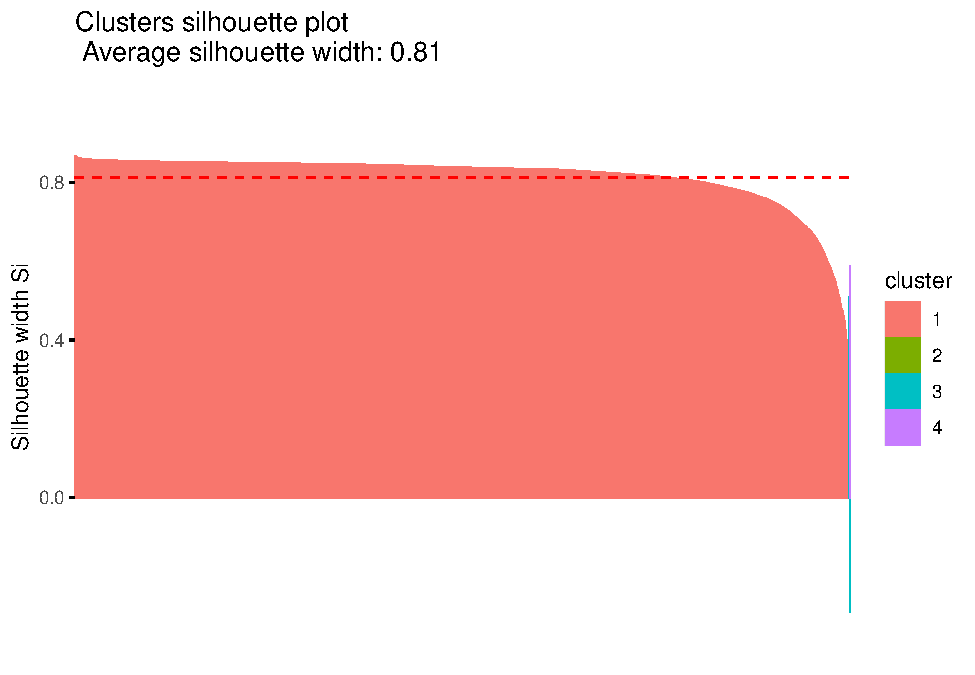
\includegraphics[keepaspectratio]{Lab2_files/figure-latex/silhouette-2.pdf}}

\begin{Shaded}
\begin{Highlighting}[]
\NormalTok{mean\_sil\_kmeans }\OtherTok{\textless{}{-}} \FunctionTok{mean}\NormalTok{(sil\_kmeans[,}\DecValTok{3}\NormalTok{])}
\NormalTok{mean\_sil\_hc }\OtherTok{\textless{}{-}} \FunctionTok{mean}\NormalTok{(sil\_hc[,}\DecValTok{3}\NormalTok{])}

\NormalTok{mean\_sil\_kmeans}
\end{Highlighting}
\end{Shaded}

\begin{verbatim}
## [1] 0.3739578
\end{verbatim}

\begin{Shaded}
\begin{Highlighting}[]
\NormalTok{mean\_sil\_hc}
\end{Highlighting}
\end{Shaded}

\begin{verbatim}
## [1] 0.8113346
\end{verbatim}

\subsubsection{Interpretación de la
silueta}\label{interpretaciuxf3n-de-la-silueta}

\begin{itemize}
\tightlist
\item
  K-means obtuvo una silueta promedio de \textbf{0.37}.
\item
  El método jerárquico obtuvo una silueta promedio de \textbf{0.81}.
\end{itemize}

Sin embargo, el clustering jerárquico generó un grupo extremadamente
dominante (19,701 películas) y varios clusters muy pequeños, incluso de
una sola observación, lo que indica un agrupamiento poco balanceado y
poco útil para segmentación real.

K-means, aunque tiene una silueta menor, generó grupos más equilibrados
y útiles para interpretación.\\
Por esta razón, se selecciona \textbf{K-means} para el análisis final.

\begin{center}\rule{0.5\linewidth}{0.5pt}\end{center}

\subsection{1.7 Interpretación de los grupos
(K-means)}\label{interpretaciuxf3n-de-los-grupos-k-means}

\begin{Shaded}
\begin{Highlighting}[]
\NormalTok{movies\_clustered }\OtherTok{\textless{}{-}}\NormalTok{ numeric\_vars}
\NormalTok{movies\_clustered}\SpecialCharTok{$}\NormalTok{cluster\_kmeans }\OtherTok{\textless{}{-}}\NormalTok{ kmeans\_result}\SpecialCharTok{$}\NormalTok{cluster}

\FunctionTok{table}\NormalTok{(movies\_clustered}\SpecialCharTok{$}\NormalTok{cluster\_kmeans)}
\end{Highlighting}
\end{Shaded}

\begin{verbatim}
## 
##    1    2    3    4 
## 9225  892  282 9322
\end{verbatim}

\begin{Shaded}
\begin{Highlighting}[]
\NormalTok{movies\_clustered }\SpecialCharTok{\%\textgreater{}\%}
  \FunctionTok{group\_by}\NormalTok{(cluster\_kmeans) }\SpecialCharTok{\%\textgreater{}\%}
  \FunctionTok{summarise\_all}\NormalTok{(mean)}
\end{Highlighting}
\end{Shaded}

\begin{verbatim}
## # A tibble: 4 x 13
##   cluster_kmeans popularity     budget    revenue runtime voteAvg voteCount
##            <int>      <dbl>      <dbl>      <dbl>   <dbl>   <dbl>     <dbl>
## 1              1      37.2   10277804.  23112887.   101.    6.43     763.  
## 2              2     163.   103110290. 401367712.   121.    6.90    7133.  
## 3              3      47.2     262218.   2577397.    85.5   6.28      73.4 
## 4              4       1.44      6794.      3963.    26.1   0.864      1.90
## # i 6 more variables: genresAmount <dbl>, productionCoAmount <dbl>,
## #   productionCountriesAmount <dbl>, actorsAmount <dbl>, castWomenAmount <dbl>,
## #   castMenAmount <dbl>
\end{verbatim}

\subsubsection{Interpretación
detallada}\label{interpretaciuxf3n-detallada}

\paragraph{🔵 Cluster 1 -- Producciones comerciales
medias}\label{cluster-1-producciones-comerciales-medias}

\begin{itemize}
\tightlist
\item
  Presupuesto promedio ≈ 10 millones
\item
  Revenue ≈ 23 millones
\item
  Popularidad ≈ 37
\item
  VoteAvg ≈ 6.4
\item
  Runtime ≈ 101 minutos
\end{itemize}

Este grupo representa películas comerciales estándar, con presupuesto
moderado y desempeño estable.\\
Son producciones típicas del mercado que generan ingresos proporcionales
a su inversión y mantienen buena aceptación del público.

\begin{center}\rule{0.5\linewidth}{0.5pt}\end{center}

\paragraph{🔴 Cluster 2 -- Grandes producciones
(Blockbusters)}\label{cluster-2-grandes-producciones-blockbusters}

\begin{itemize}
\tightlist
\item
  Presupuesto ≈ 103 millones
\item
  Revenue ≈ 401 millones
\item
  Popularidad ≈ 163
\item
  VoteCount ≈ 7,133
\item
  Runtime ≈ 121 minutos
\end{itemize}

Este cluster corresponde claramente a películas tipo blockbuster.\\
Son producciones de alto presupuesto, alta popularidad y altos
ingresos.\\
Representan el segmento más rentable y estratégico del mercado
cinematográfico.

\begin{center}\rule{0.5\linewidth}{0.5pt}\end{center}

\paragraph{🟢 Cluster 3 -- Cine independiente / Bajo
presupuesto}\label{cluster-3-cine-independiente-bajo-presupuesto}

\begin{itemize}
\tightlist
\item
  Presupuesto ≈ 262 mil
\item
  Revenue ≈ 2.5 millones
\item
  Popularidad ≈ 47
\item
  VoteAvg ≈ 6.28
\item
  VoteCount bajo
\end{itemize}

Este grupo representa películas de bajo presupuesto pero con buena
recepción crítica.\\
Probablemente corresponden a cine independiente o producciones de nicho.

\begin{center}\rule{0.5\linewidth}{0.5pt}\end{center}

\paragraph{🟣 Cluster 4 -- Producciones marginales o muy
pequeñas}\label{cluster-4-producciones-marginales-o-muy-pequeuxf1as}

\begin{itemize}
\tightlist
\item
  Presupuesto ≈ 6,794
\item
  Revenue ≈ 3,963
\item
  Popularidad ≈ 1.44
\item
  VoteAvg ≈ 0.86
\item
  Runtime ≈ 26 minutos
\end{itemize}

Este cluster agrupa producciones de muy bajo impacto comercial.\\
Podrían tratarse de cortometrajes, proyectos experimentales o
producciones no comerciales.

\begin{center}\rule{0.5\linewidth}{0.5pt}\end{center}

\subsubsection{Conclusión del
Clustering}\label{conclusiuxf3n-del-clustering}

El análisis permitió identificar cuatro segmentos claramente
diferenciados dentro del mercado cinematográfico:

\begin{enumerate}
\def\labelenumi{\arabic{enumi}.}
\tightlist
\item
  Blockbusters altamente rentables\\
\item
  Producciones comerciales medianas\\
\item
  Cine independiente con buena crítica\\
\item
  Producciones marginales de bajo impacto
\end{enumerate}

Esta segmentación puede ayudar a CineVision Studios a definir
estrategias de inversión y diversificación de mercado.

\section{2. Tipo de Variables}\label{tipo-de-variables}

\subsection{Variables Cuantitativas}\label{variables-cuantitativas}

\begin{itemize}
\tightlist
\item
  id → Cuantitativa, discreta\\
\item
  budget → Cuantitativa, discreta\\
\item
  revenue → Cuantitativa, discreta\\
\item
  runtime → Cuantitativa, discreta\\
\item
  popularity → Cuantitativa, continua\\
\item
  voteAvg → Cuantitativa, continua\\
\item
  voteCount → Cuantitativa, discreta\\
\item
  genresAmount → Cuantitativa, discreta\\
\item
  productionCoAmount → Cuantitativa, discreta\\
\item
  productionCountriesAmount → Cuantitativa, discreta\\
\item
  actorsAmount → Cuantitativa, discreta\\
\item
  castWomenAmount → Cuantitativa, discreta\\
\item
  castMenAmount → Cuantitativa, discreta\\
\item
  releaseYear → Cuantitativa, discreta
\end{itemize}

\subsection{Variables Cualitativas
Nominales}\label{variables-cualitativas-nominales}

\begin{itemize}
\tightlist
\item
  genres\\
\item
  homePage\\
\item
  productionCompany\\
\item
  productionCompanyCountry\\
\item
  productionCountry\\
\item
  video\\
\item
  director\\
\item
  actors\\
\item
  actorsCharacter\\
\item
  originalTitle\\
\item
  title\\
\item
  originalLanguage
\end{itemize}

\subsection{Variables Cualitativas
Ordinales}\label{variables-cualitativas-ordinales}

\begin{itemize}
\tightlist
\item
  actorsPopularity\\
\item
  releaseDate
\end{itemize}

\begin{center}\rule{0.5\linewidth}{0.5pt}\end{center}

\end{document}
